\documentclass[12pt,a4paper]{article}
\usepackage[marginparsep=8pt,left=2.5cm,right=2.5cm,top=2.5cm,bottom=3cm]{geometry}
\usepackage{graphicx}
\usepackage[czech]{babel}
\usepackage[utf8]{inputenc}
\usepackage{amsmath}
\usepackage[dvipsnames]{xcolor}
%\setlength{\parindent}{0pt}% Remove paragraph indent
\graphicspath{ {./images/} }
\newcommand*\rfrac[2]{{}^{#1}\!/_{#2}}

\newcommand{\overbar}[1]{\mkern 2.5mu\overline{\mkern-2.5mu#1\mkern-2.5mu}\mkern 2.5mu}

\usepackage[explicit]{titlesec}
\titleformat{\section}{\bf\Large}{#1}{1em}{}
\titleformat{\subsection}{\bf\large}{#1}{1em}{}

\pagenumbering{gobble} % da pryc cislo stranky na uvodni strance..

\usepackage{listings}
\lstset{
  language=Python,
  keywordstyle=\ttfamily\color{MidnightBlue},
  emph={MyClass,__init__},
  emphstyle=\ttfamily\color{Mahogany},  
  stringstyle=\color{OliveGreen},
  basicstyle=\ttfamily,
  columns=fullflexible,
  breaklines=true,
  postbreak=\mbox{\textcolor{red}{$\hookrightarrow$}\space},
  frame=tb,      
}

%% ZAHLAVI A ZAPATI
\usepackage{fancyhdr}
\pagestyle{fancy}
\renewcommand{\sectionmark}[1]{\markright{#1}}

% prostredni cast zapati
\cfoot{\thepage}

% leva cast zahlavi -- nazev sekce/subsekce
\lhead{\fancyplain{}{\rightmark}}

% prava cast zahlavi -- logo fitu

\rhead{
\includegraphics[width=4cm]{logo}}

%% PROKLIKAVATELNE ODKAZY -- nastaveni xetex/pdftex
\usepackage[pdftex,pdfpagelabels,bookmarks,hyperindex,hyperfigures]{hyperref}

\hypersetup{
  colorlinks,
  citecolor=blue,
  filecolor=blue,
  linkcolor=blue,
  urlcolor=blue
}

\begin{document}

\begin{titlepage}
  % pro zobrazeni loga v zahlavi
  \thispagestyle{fancy}

  % vertikalni zarovnani
  \vspace*{\fill}
  \begin{center}
    {\fontsize{20}{30}\selectfont BI-PST 2018}\\[1cm]
    {\fontsize{30}{100}\selectfont \textbf{Domácí Úkol}}\\[4.2cm]
  \end{center}

  % vertikalni zarovnani
  \vspace*{\fill}

  % seznam clenu tymu razeny abecedne podle krestniho jmena
  {\fontsize{10}{10} \selectfont \noindent
  \textbf{Autoři:}\\
  Pavel Jahoda a Jan Lidák
  }
\end{titlepage}

%%%%% 
\renewcommand{\headrulewidth}{0.4pt}
\renewcommand{\footrulewidth}{0.4pt}

% rimska cisla pro cislovani stranek v obsahu
\pagenumbering{roman}

% samotne vlozeni obsahu
\tableofcontents

\newpage

% zapnout bezne cislovani stranek pomoci arabskych cislic
\pagenumbering{arabic}

\section{Úvod}
\subsection{Výběr reprezentanta}
Jako reprezentant byl zvolen Pavel Jahoda.\\
$K = 8$\\
$L = 6$\\
$M = ((8+6)*47) mod 11 + 1 = 10$\\
Zpracovávali jsme tedy dataset získaný pozorováním vrabců během zimy (ex0221).
\subsection{Nástroje}
Použili jsme programovací jazyk Python (verze 3) a knihovny numpy, pandas, scipy, statsmodels a matplotlib.
\subsection{Ukázka kódu}
Zpráva obsahuje jen malou část použitého kódu. Celý kód si je možné prohlédnout na adrese \url{https://www.dropbox.com/s/sqmylamw36kz9z2/main.py?dl=0}.
\pagebreak

\section{Úkol 1 - Načtení a popis datasetu}
Data jsou z pozorování 59 vrabců během zimy. První veličina {\bf X} reprezentuje váhy vrabců v gramech. Druhá veličina {\bf Y} nabývá dvou hodnot 'survived', pokud vrabec přežil a 'perished' pokud nepřežil. Sledovanou proměnnou X jsme rozdělili na dvě pozorované skupiny takzvaných \textit{independent and identically distributed random variables}. Tedy v každé skupině jsou náhodné veličiny reprezentující výsledky pokusu prováděného za stejných podmínek.  {\bf X1} jsou vrabci co přežili a je jich 35. {\bf X2} jsou vrabci co nepřežili a je jich 24.\\
EX1=25.463, var(X1)=1.539 a medián je 25.7.\\
EX1=26.275, var(X2)=2.078 a medián je 26.\\
\par \medskip
\flushleft{Data se načetla následujícími python příkazy:\par \medskip}
\begin{lstlisting}
data = pandas.read_csv(dataPath, sep=';').replace({'perished' : 0, 'survived' : 1})
return numpy.array(data.loc[data.Status == 1].Weight), np.array(data.loc[data.Status ==0].Weight)
\end{lstlisting}

\section{Úkol 2 - Hustota a distribuční funkce}
Nejprve vykreslíme histogram a poté graf distribuční funkce odhadnutý z grafu empirické distribuční funkce pro vrabce kteří přežili.\\
Graf distribuční funkce byl odhadnutý následujícím příkazem:\par \medskip
\begin{lstlisting}
from statsmodels.distributions.empirical_distribution import ECDF
ecdf = ECDF(weightsSurvived)
\end{lstlisting}
\smallskip
\noindent 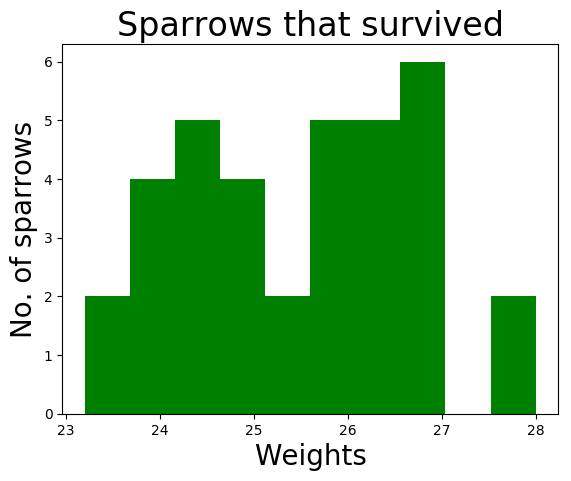
\includegraphics[width=3.1in]{survivedHist}
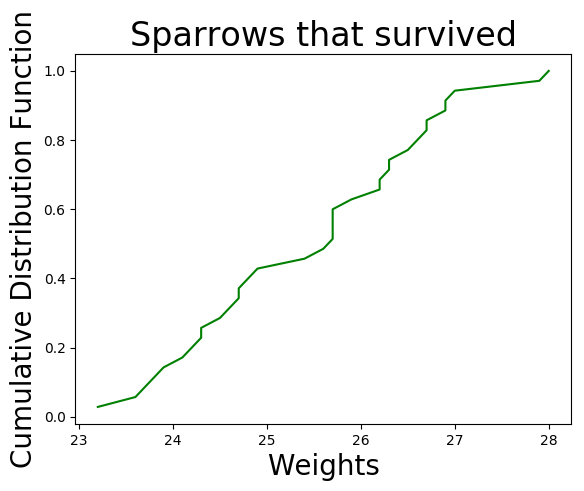
\includegraphics[width=3.1in]{survivedDist}
\pagebreak

Poté vykreslíme histogram a graf distribuční funkce funkce pro vrabce kteří nepřežili a to obdobným způsobem jako pro vrabce kteří přežili.\\
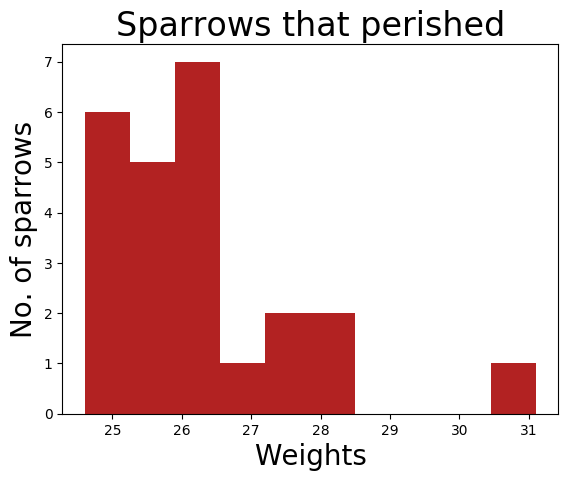
\includegraphics[width=3.1in]{diedHist}
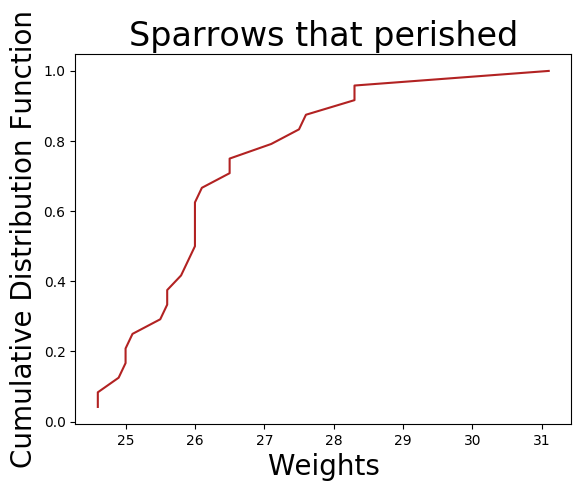
\includegraphics[width=3.1in]{diedDist}
Graf empirické distribuční funkce se podobá grafu exponenciálního rozdělení s parametrem $\lambda$ = 1.\par \bigskip
\pagebreak

\section{Úkol 3 - Nejbližší rozdělení}
Histogram přeživších vrabců byl nejprve znormován, tak aby obsah histogramu byl roven 1 pro lepší porovnání s grafy rozdělení, jejichž obsah pod křivkou je také roven 1. Po zanesení normálního, exponenciálního a rovnoměrného rozdělení s odhadnutými parametry do grafů histogramu vidíme, že histogram nejvíce odpovídá normálnímu rozdělení.
\begin{center}
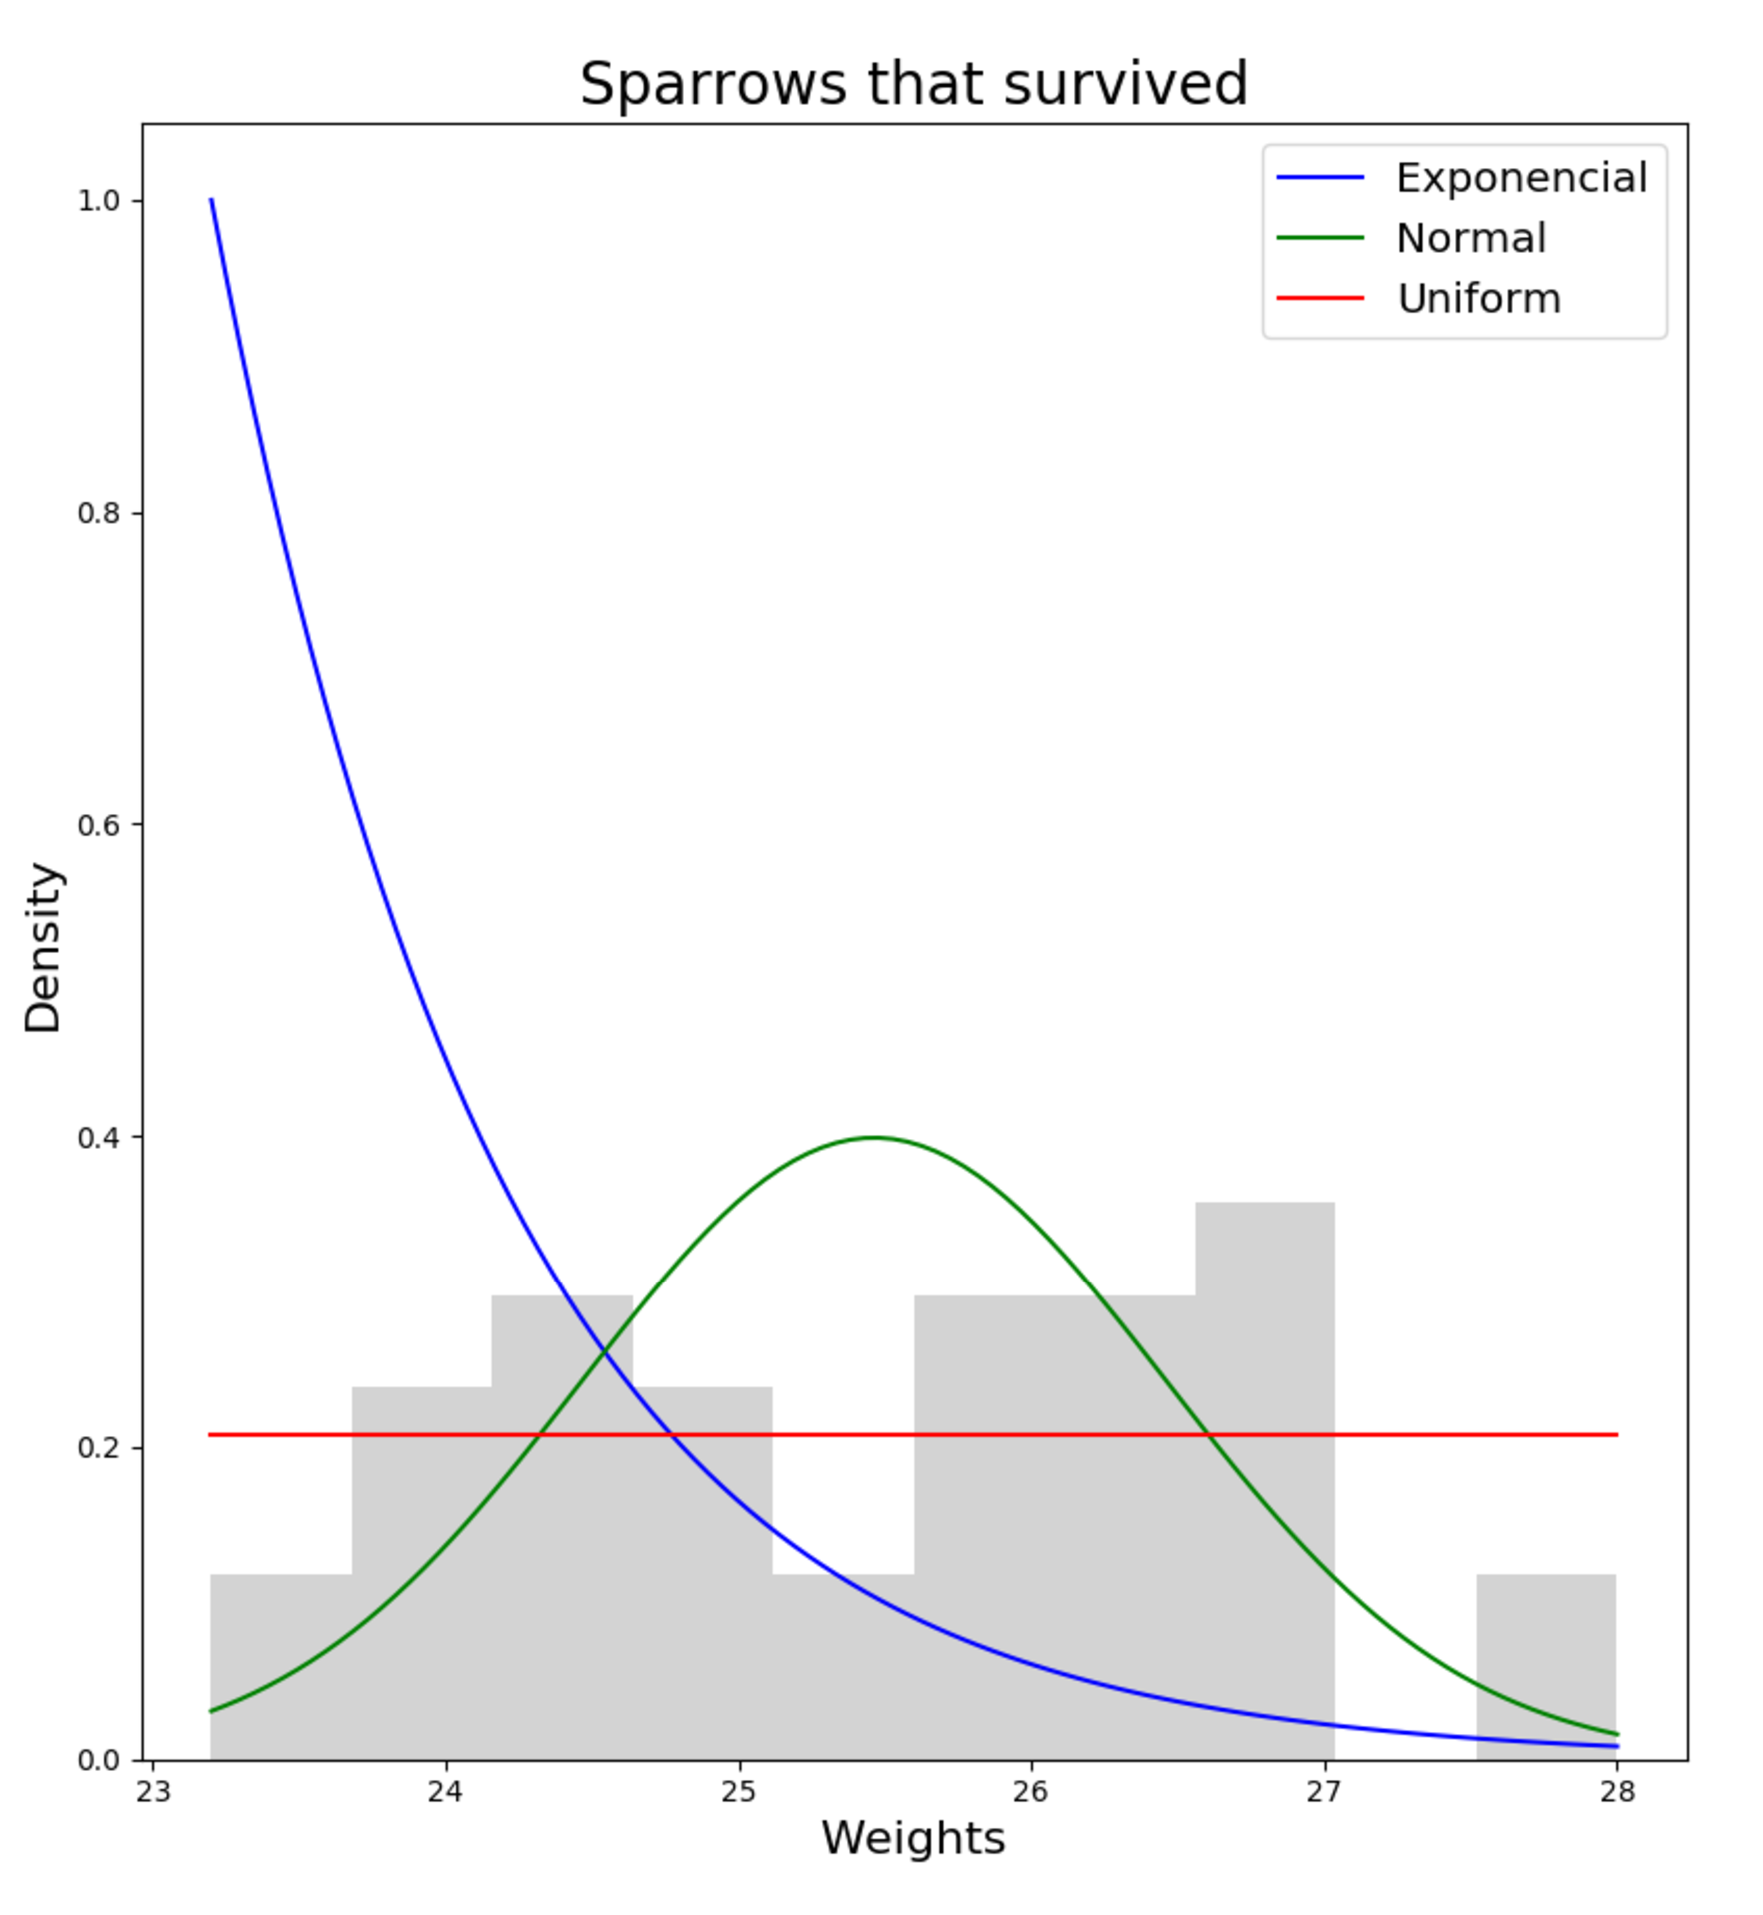
\includegraphics[width=5in]{3_survived}
\end{center}
Příkazy na získaní hodnot exponenciální a normální funkce, které jsou vykresleny do histogramu výše:\par \medskip
\begin{lstlisting}
from scipy import stats
x1 = np.linspace(min(weightsSurvived),max(weightsSurvived),100)
exponencialX1 = stats.expon.pdf(x1,scale=1,loc=min(weightsSurvived))
normalDistributionX1 = stats.norm.pdf(x1,loc=EX1)
\end{lstlisting}
\pagebreak
Určení, které rozdělení odpovídá nejlepé grafu vrabců, kteří zimu nepřežili je obtížnější, jelikož to není visuálně patrné. První způsob, který jsem použil na zjištění nejbližšího rozdělení bylo spočítat součet rozdílu mezi výškami sloupců histogramů a hodnotami funkcí pro x rovno středu daného sloupce. V tomto způsobu vyšlo normální rozdělení jako rozdělení které histogramu více odpovídá ( 0.73 normalání a 0.94 exponenciální). Dále mi co se zjištění podobnosti přišlo přirozené penalizovat extrémní rozdíli  mezi mezi výškami sloupců histogramů a hodnotami funkcí. Umocnění rozdílu zapříčiní požadovanou penalizaci. V tomto případě vyšla výsledná suma normálního rozdělení 0.13 oproti 0.20 u exponenciálního rozdělení, tudíž si myslíme, že normální rozdelení je nejvíce podobné histogramu zemřelých vrabců. Statistická významnost tohoto tvrzení se stejně jako u vrabců kteří přežili odvíjí od počtu náhodných veličin, kterých je 24 (nepřežili) a 35 (přežili).
\begin{center}
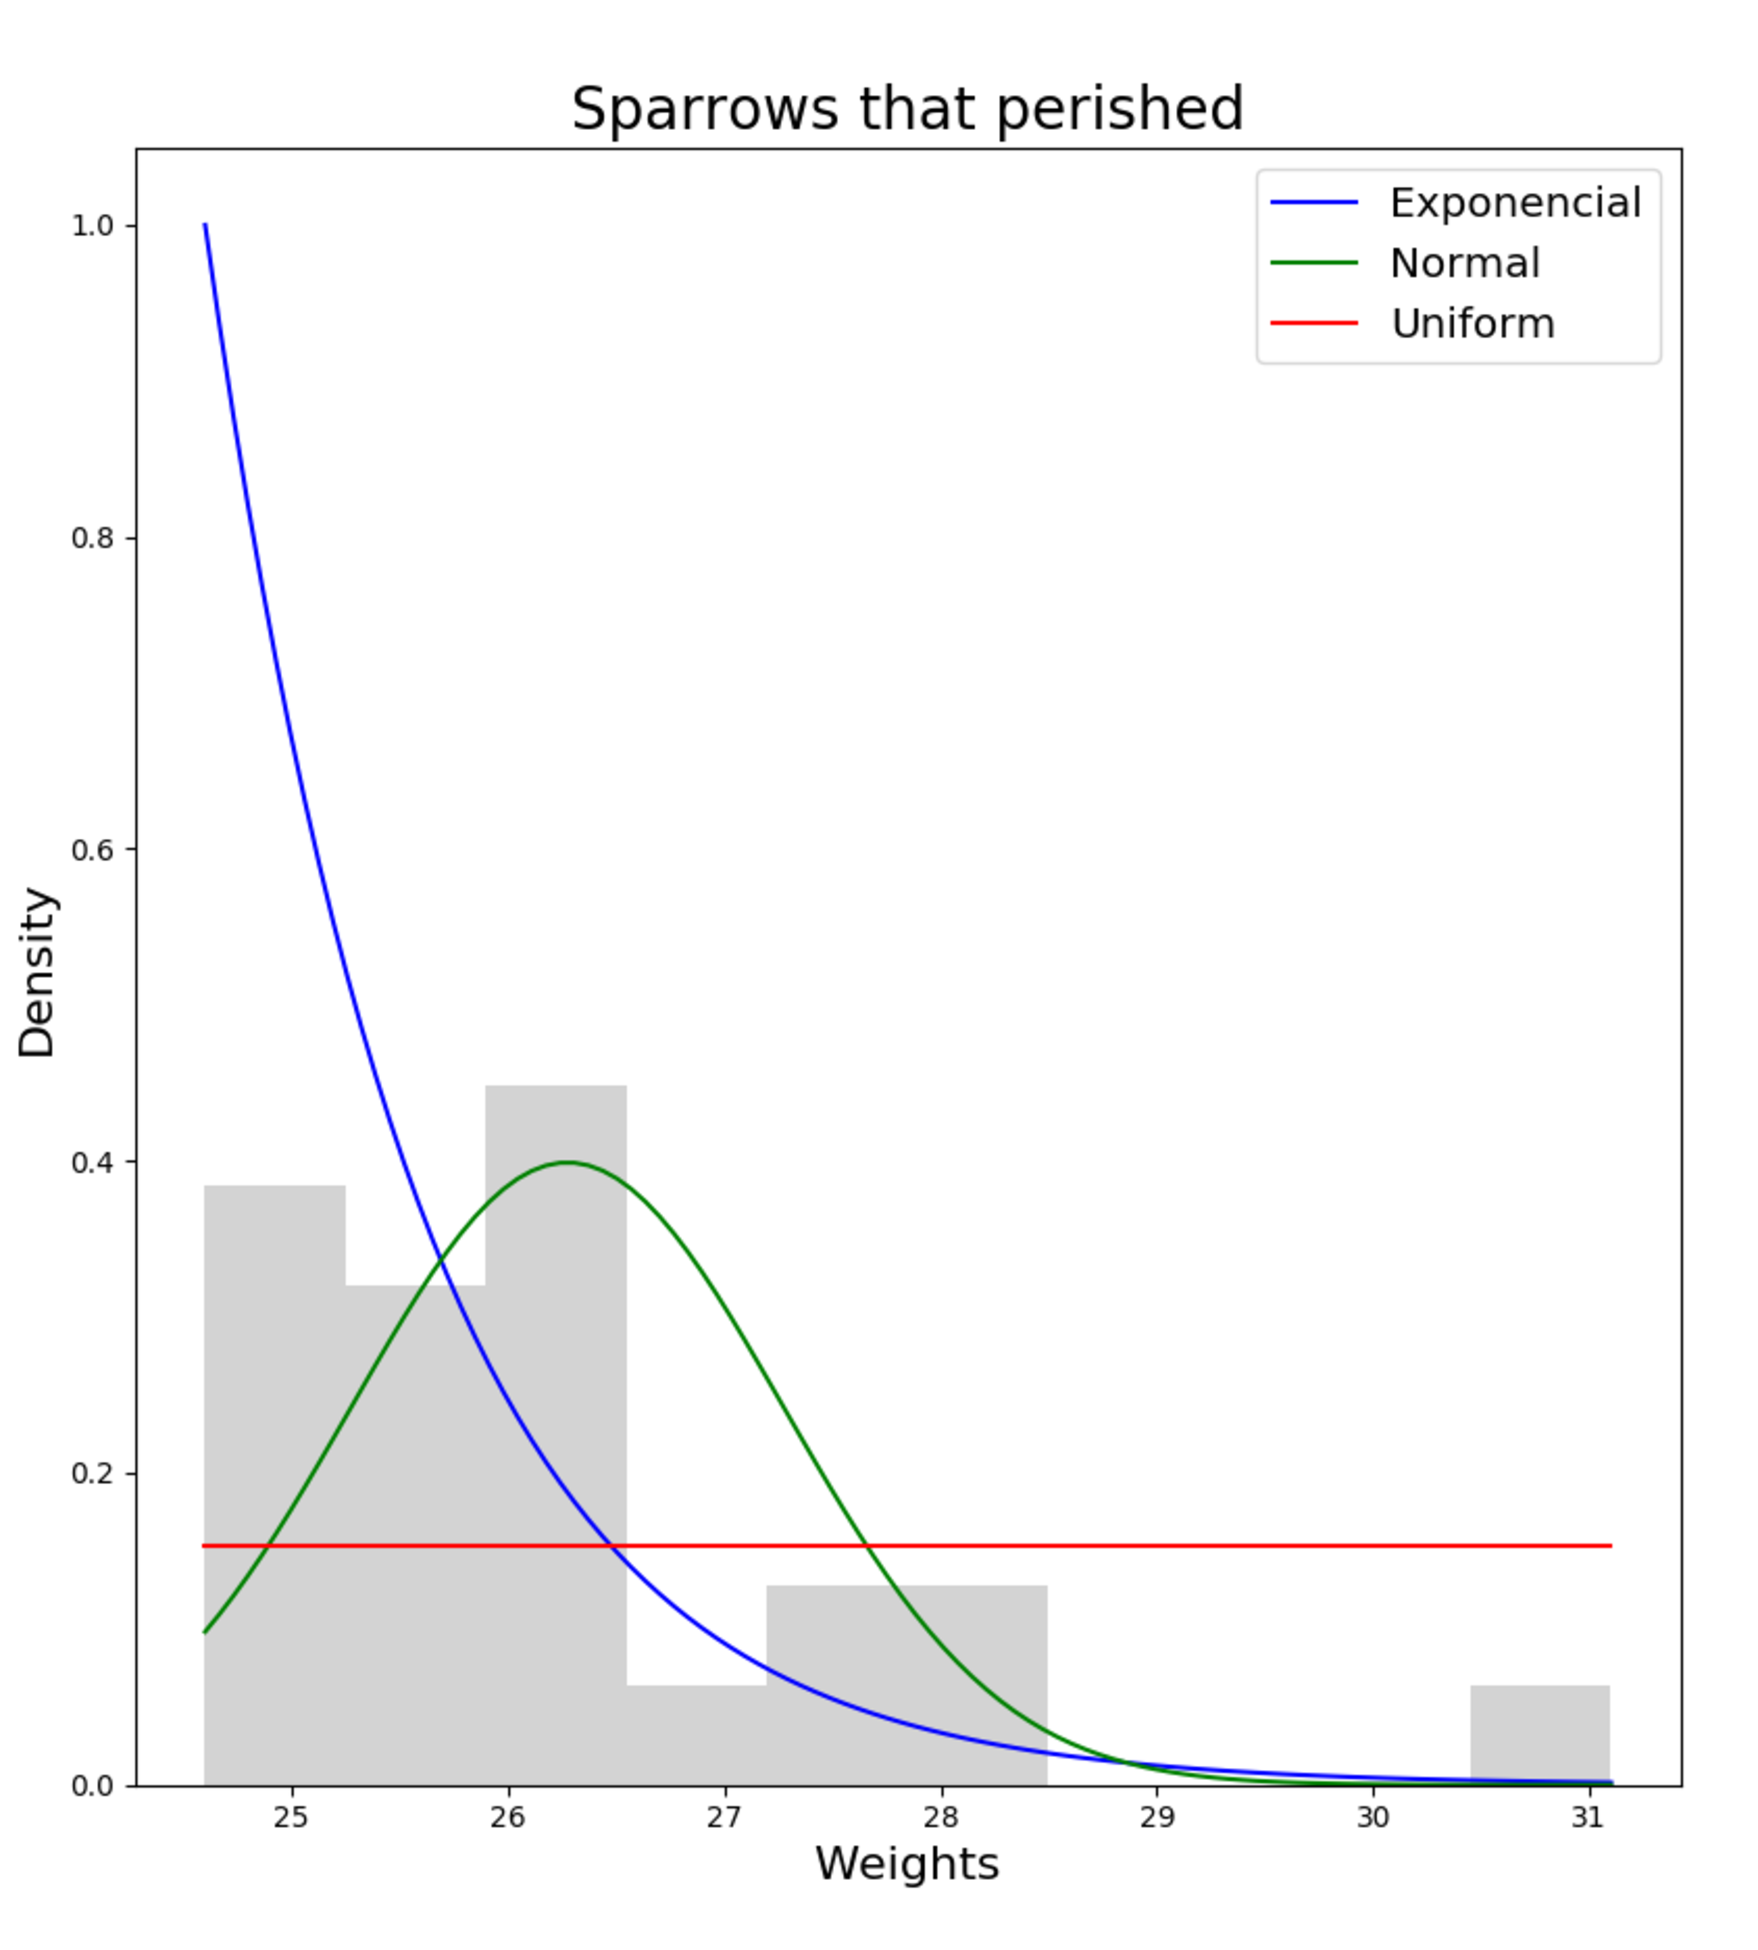
\includegraphics[width=5in]{3_died}
\end{center}
\pagebreak

\section{Úkol 4 - Generování náhodného výběru}
Na následujících grafech je zobrazeno 100 vygenerovaných hodnot spolu s načtenými daty z datasetu. Histogram přeživších vrabců připomíná normálního rozdělení s parametry $\lambda$ = EX = 25.793 a $\sigma ^2$ = varX = 1.918, hodnoty byli tedy generovány s těmito parametry. 

První graf vygenerovaných dat poměrně silně připomíná získaná data, věříme tedy že toto rozdělení bylo zvoleno správně.

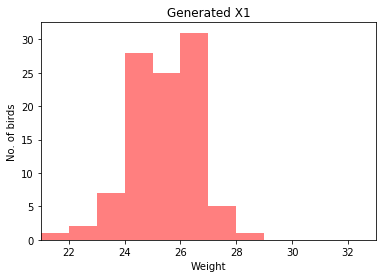
\includegraphics[width=3.1in]{4_Survived_Gen}
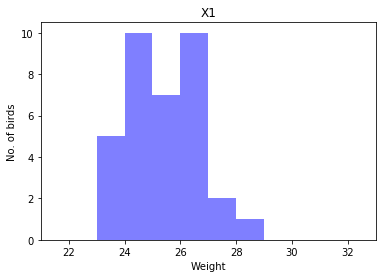
\includegraphics[width=3.1in]{4_Survived_Data}

Histogram vrabců jež nepřežili se také podobá normálnímu rozdelení, a to s parametry $\lambda$ = EX = 26.275 a $\sigma ^2$ = varX = 2.078. Data byla generována jako normální normální rozdělení s těmito parametry.

Data vygenerovaná pro mrtvé opeřence už na tom jsou hůře. Generovaná data jsou oproti naměřeným datům poněkud rozlezlé, zde by se hodilo mít větší dataset aby se dala lépe odhadnout distribuční funkce, popřípadě parametry rozdělení.

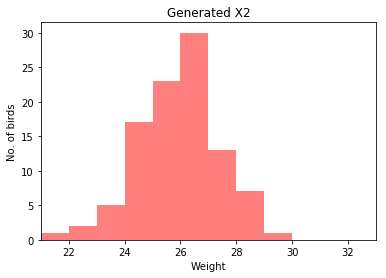
\includegraphics[width=3.1in]{4_Died_Gen}
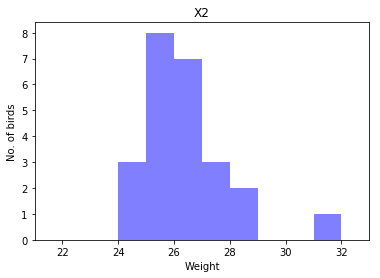
\includegraphics[width=3.1in]{4_Died_Data}

\pagebreak

\section{Úkol 5 - Konfidenční interval}

Jelikož neznáme rozptyl našich rozdělení (pouze je dokážeme odhadnout) použijeme pro výpočet konfidenčních intervalů namísto rozptylu $\sigma$ výběrový rozptyl $s_n$. Dále $\bar{X}_n$ je výběrový průměr veličiny, $t_{\alpha/2,n-1}$ je kritická hodnota Studentova t-rozdělení, n je počet prvků v rozdělení. Veličina X1 jsou vrabci jež přežili, X2 vrabci co nepřežili.  Spolehlivost má být 95\%, tedy $\alpha = 0.05$.

Oboustranný 95\% konfidenční interval pro X1 spočteme jako:

\begin{gather}
\begin{align}
(S_{X1},U_{X1})
= (\overbar{X1}_{n_1} - t_{\alpha/2,n_1-1}.\frac{s_{n_1}}{\sqrt{n_1}},
   \overbar{X1}_{n_1} + t_{\alpha/2,n_1-1}.\frac{s_{n_1}}{\sqrt{n_1}}) \nonumber\\
= (25,46 - 2,03.\frac{1,59}{5,9},
   25,46 + 2,03.\frac{1,59}{5,9})
= \textbf{(25.031, 25.895)}
\end{align}
\end{gather}\\

Oboustranný 95\% konfidenční interval pro X2:

\begin{align}
(S_{X2},U_{X2}) = 
(\overbar{X2}_{n_2} - t_{\alpha/2,n_2-1}.\frac{s_{n_2}}{\sqrt{n_2}},
 \overbar{X2}_{n_2} + t_{\alpha/2,n_2-1}.\frac{s_{n_2}	}{\sqrt{n_2}}) \nonumber\\
= (26,275 - 2,06.\frac{2,17}{4,9},
   26,275 + 2,06.\frac{2,17}{4,9})
= \textbf{(25.656, 26.894)}
\end{align}

\section{Úkol 6 - Testování hypotézy}
Testujeme hypotézu, zda je střední hodnota rovna hodnotě K (parametr úlohy).\\[0.4cm]
$H_0$ : $\mu = K$\\
$H_A$ : $\mu \neq K$\\
$K = 8$\\
$\alpha = 0.05$\par \medskip
\textbf{Vrabci co prežili}\\
Jelikož $K \notin (25.031, 25.895)$ přijímáme alternatívní hypotézu $H_A$, která říká, že střední hodnota vah vrabců kteří přežili se nerovná K.
\par \medskip
\textbf{Vrabci co neprežili}\\
Jelikož $K \notin (25.656, 26.894)$ přijímáme alternatívní hypotézu $H_A$, která říká, že střední hodnota vah vrabců kteří nepřežili se nerovná K.
\pagebreak

\section{Úkol 7 - Testování středních hodnot}
Testujeme hypotézu, zda se rovnají střední hodnoty vah vrabců jež přežili a zahynuli. Alternativa k této hypotéze bude, že střední hodnota se u přeživších a mrtvých vrabců liší.

$H_0: \mu_p = \mu_z$

$H_A: \mu_p \neq \mu_z$

$\alpha = 0,05$\\

Pro srovnání použijeme dvouvýběrový t-test s předpokladem, že rozptyl obou veličin je stejný. p-hodnota nám vyšla 0.027 $<$ 0.05. Hypotézu $H_0$ lze tedy zamítnout ve prospěch alternaticní hypotézy $H_A$, že \textbf{vrabci mají rozdílnou střední hodnotu vah v závislosti na tom zda přežili či nikoliv.} \\

Abychom si byli jisti že jsme zvolili správnou variantu t-testu, otestujeme ještě rozptyl veličin pomocí Bartlettova testu. p-hodnota = 0.41 $>$ 0.05, takže shodu rozptylů výšek na hladině významnosti 5\% nezamítáme, a potvrzuje naši volbu.\par \bigskip
\flushleft{Pro zjištění p-hodnot použitím dvouvýběrového t-testu a Bartlettova testu byl použit následující kód:\par \medskip}
\begin{lstlisting}
from scipy import stats
p_value1 = stats.ttest_ind(weightsSurvived, weightsDied, equal_var=True)
p_value2 = stats.bartlett(weightsSurvived, weightsDied)
\end{lstlisting}


\end{document}

